\documentclass[9pt,twocolumn,twoside]{../../styles/osajnl}
\usepackage{fancyvrb}
\journal{i524} 

\title{Analysis of USGS Earthquake Data}

\author[1,*]{Nandita Sathe}

\affil[1]{School of Informatics and Computing, Bloomington, IN 47408, U.S.A.}

\affil[*]{Corresponding authors: nsathe@iu.edu}

\dates{project-001, \today}

\ociscodes{I524, geospatial, MongoDB, Plotly, K-means clustering, DBSCAN, Python, pymongo, USGS, Ansible, Cherrypy}

\doi{\url{https://github.com/cloudmesh/sp17-i524/blob/master/project/S17-IO-3017/report/report.pdf}}


\begin{abstract}
US Geological Survey's (USGS) Earthquake Hazards Program monitor and report earthquakes, assess earthquake impacts and hazards, and research the causes and effects of earthquakes \cite{www-usgs1}. The geo-spatial data it collects is available for free. Big Data Analytics tools are used to analyze this data. Machine learning algorithms are used for advanced data analysis and earthquakes prediction.
\newline
\end{abstract}

\setboolean{displaycopyright}{true}

\begin{document}

\maketitle

\section{Introduction}

USGS collects volumes of geospatial data pertaining to earthquakes and makes it available for analysis. The project obtains a chunk of the data using GeoJSON web service provided by USGS. The data is saved locally in MongoDB database. Data is analysed using machine learning algorithms. The output is plotted (rendered) on web browser. A light weight web server is used to respond to the web requests. Project is capable of running in cloud environment. Deployment is automated using Ansible. 

\section{Technologies Used}

Technologies used for development and deployment of this project are listed below.
\begin{enumerate}

\item {\bf Cloudmesh} - Cloudmesh provides Cloud Testbeds as a Service (CTaaS). It is a platform where one can manage all cloud accounts and local files enabling one to copy them between services. Project uses cloudmesh to connect to various cloud environments.

\item {\bf Ansible} - Ansible is an IT automation tool that automates cloud provisioning, configuration management, and application deployment. Once Ansible gets installed on a control node, which is an agentless architecture, it connects to a managed node through the default OpenSSH connection type. Ptoject uses ansible for one-click deployment.

\item {\bf Python} - Python is an object oriented, light weight programming language. Python is primary programming language used in this project.

\item {\bf Mongo-DB} - MongoDB is an unstructured (NOSQL) database, which uses document-oriented data model. It stores data in flexible JSON-like documents. The project uses Mongo-DB to store GeoJSON data of earthquakes locally.

\item {\bf Plotly} - Plotly is data analytics and visualization tool. One can create interactive graphs using plotly. It provides graphing libraries for Python. The plotly is used in the project as a visualization tool.

\item {\bf Scikit-learn} - Scikit-learn provides tools for data analysis and data mining. Scikit-learn provides a wide range of learning algorithms. Scikits are the names given to the modules for SciPy, a fundamental library for scientific computing. As these modules provide different learning algorithms, the library is named as sciki-learn. In this project data classification is done using scikit learn.

\item {\bf Cherrypy} - CherryPy is an object-oriented web application framework. It is designed for rapid development of web applications by wrapping the HTTP protocol. It is WSGI (Web Server Gateway Interface) thread-pooled web server. Cherrypy is used as a web server in the application.
\end{enumerate}

\section{Design}

Figure 1 shows main components and data flow of the application. There are four major components in the application.

\begin{figure}[htbp]
\centering
\fbox{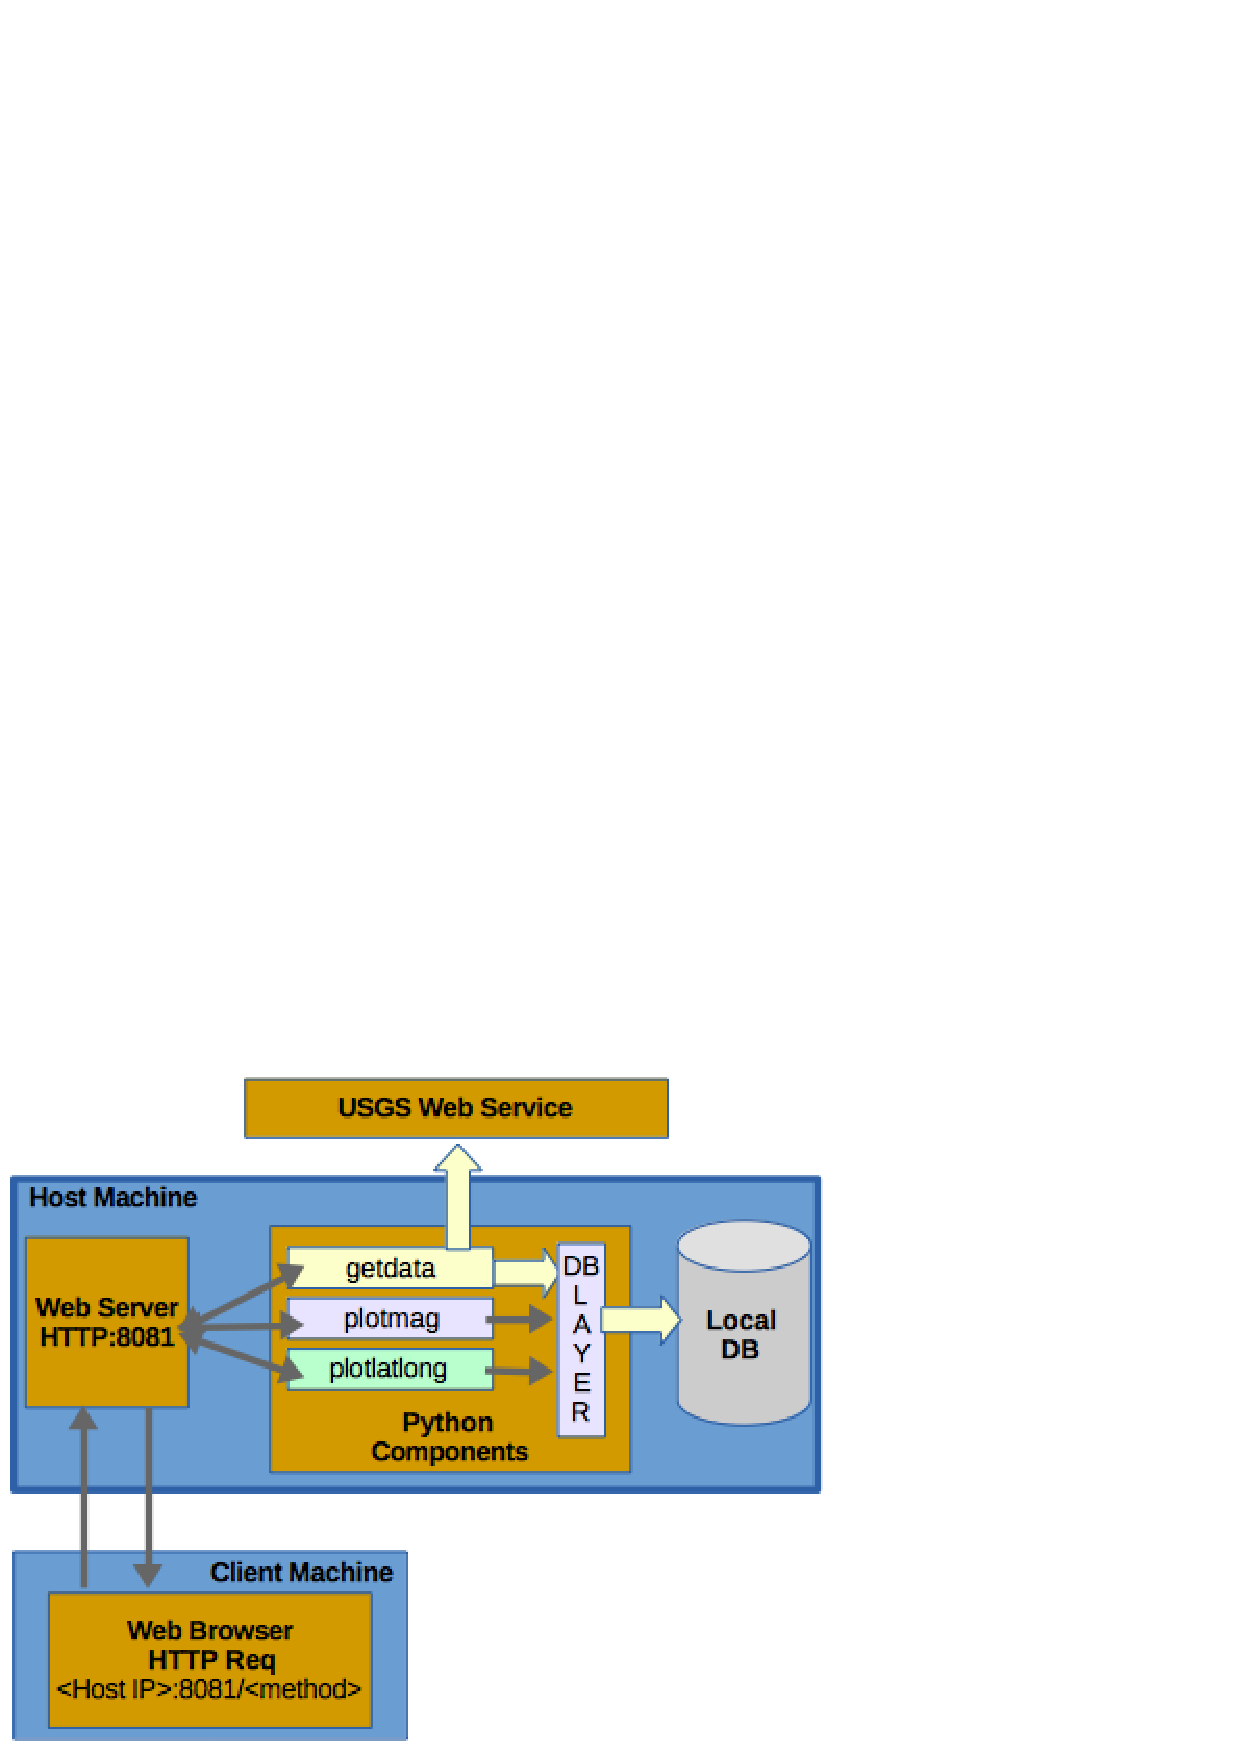
\includegraphics[width=\linewidth]{images/figure4}}
\caption{Application Components} 
\label{fig:figure4}
\end{figure}

\subsection{WebServer}
Purpose of web server is to listen to the user's HTTP GET request, call appropriate python method at the backend, get the response from the python method, and send it to the web client as a response. The server listens at port 8081.

\subsection{getusgsdata - getdata}
getusgsdata component is responsible for fetching the data from USGS and storing it in local database. It uses dblayer common component to communicate with the local database. Running this component at least once is necessary as it downloads the data on which other components are dependent. 

\subsection{kmeansplot - plotmag}
kmeansplot component implements the K-Means clustering algorithm and plots it using plotly library. It reads the Magnitude and Depth data from local database using dblayer common component. The algorithm classifies the data in 3 clusters based on the earthquakes magnitudes. Number 3 is selected by trial and error basis. 
Output of plotly.plot() function is set as \emph div so that it returns the \emph div with scatter plot and data, which has later been embedded into a simple HTML. This HTML is rendered on web browser as output.

\subsection{dbscanplot - plotlatlong}
dbscanplot implements DBSCAN algorithm for clustering the latitude-longitude data. It reads the data from local database using dblayer common component. 
Clusters are plotted on a globe using plotly's Scattergeo() function. Following programming statements ensure showing North and South America region on globe.

\[ geo=dict(scope=('north america', 'south america') \]
\[projection=dict(type='orthographic') \]

For clustering lat long data DBSCAN algorithm is used instead of K-Means because, (1) for clustering lat long data it needs an algorithm that can handle arbitrary distance function, (2) K-Means works well with linear data. Lat long data is not linear, (3) Unlike K-Means, number of clusters are not required to mention in DBSCAN. It is hard to predict clusters when locations are spread across world.

\section{Implementation}

\subsection{USGS Web Service and Data Set}
USGS earthquake data is fetched using the USGS web service and passing relevant parameters to it. Out of the voluminous world-wide data of decades this project uses data of earthquakes appeared in North and South America for duration of 2 years from 2015-1-1 till 2017-1-1, having magnitude over 4. To select North and South America region data, its Latitude and Longitude are taken from Search Earth Catalog tool provided by USGS. \cite{www-usgs3}. Web service returns data in JSON format.

\subsection{Data Processing and Visualization}

{\bf Severity of earthquakes.} Severity of earthquakes is analysed by their magnitude and depth. Data is classified into clusters using K-Means clustering algorithm (Section 4.1). Clusters are plotted on a interactive scatter plot.

{\bf Region affected the most by earthquakes}. Analysing Latitude-Longitude of epicenter of the earthquake shows the regions where earthquakes are frequent. Lat-long data is clustered using DBSCAN algorithm (Section 4.2). Clusters are plotted on a geo-scatter plot on a world map.

\subsection{Deployment}

Project is deployed using ansible. Ansible jobs are collected in a playbook and run on virtual clusters provided by Chameleon and Jetstream cloud. The tasks include cloning the git repository, installing software stack, installing dependencies and installing MongoDB.

\subsection{Local Data Storage}
To avoid frequent web service calls and unnecessary traffic, data once downloaded, is stored locally in MongoDB for further usage by other components. Data is fetched using pymongo library. 

\subsection{Steps to Execute}

Steps to execute the project are explained in detail in README.md file \cite{readme-001}.

\section{Clustering Algorithms}

\subsection{K-Means Clustering}
Given a target number, \emph k, of clusters to find, K-means algorithm locates the centers of each of those \emph k clusters and the boundaries between them. It does this using the following algorithm \cite{www-kmeans}.
\begin{itemize}
    
    \item Step 1: Start with a randomly selected set of \emph k centroids 

    \item Step 2: Determine which observation is in which cluster, based on which centroid it is closest to (using the squared Euclidean distance. 
    \[   \sum_{j=1}^p (x_{ij} - X_{i^1j})^2   \]
    
    where \emph p is the number of dimensions)
    
    \item Re-calculate the centroids of each cluster by minimizing the squared Euclidean distance to each observation in the cluster
    
    \item Repeat 2. and 3. until the members of the clusters (and hence the positions of the centroids) no longer change.

\end{itemize}

\subsection{DBSCAN}
DBSCAN (Density-Based Spatial Clustering of Application with Noise) is a clustering algorithm. Given a set of points in some space, it groups together points that are closely packed together (points with many nearby neighbors), and marks points as outliers if they lie alone in low-density regions. Unlike K-Means Clustering, DBSCAN doesn't need to specify the number of clusters as it finds all the clusters that satisfy the requirement. Following points summarize the algorithm \cite{www-dbscan}.

\begin{itemize}
    \item Step 1: For each point in the data set, an n-dimensional sphere of radius \emph epsilon is drawn around the point (if you have n-dimensional data).
    
    \item Step 2: If the number of points inside the sphere is larger than \emph min-samples, the center of the sphere is set as a cluster, and all the points within the sphere belong to this cluster.
    
    \item Step 3: Loop through all the points within the sphere with the above 2 steps, and expand the cluster whenever it satisfy the 2 rules.
    
    \item Step 4: For the points, which do not belong to any cluster, are treated as outliers. 
\end{itemize}


\section{Benchmarking}

The performance of application was tested on the speed and latency while data input/output and data processing. Two different sized datasets were used for testing. They are given in Table 'Datasets'. The Table 'VM Configuration' shows details of VMs used for performance testing. Results are shown in Table 'Benchmark Results'.
 

\begin{table}[htbp]
  
%\begin{left}
\caption{\bf VM Configuration}
\begin{tabular}{ m{5em} m{2cm} m{2cm} } 
\hline
Cloud & Chameleon & Jetstream \\ 
Image & Ubuntu-Server-14.04-LTS & ubuntu-14.04-trusty-server-cloudimg \\ 
Group & pearth & pearth \\ 
Flavour & m1.small & m1.small \\ 
Assign Floating IP & True & True \\ 

\hline
\end{tabular}
%\end{left}
\end{table} 

\begin{table}[htbp]
%\begin{left}
\caption{\bf Datasets}
\begin{tabular}{ m{5em} m{2cm} m{2cm} } 
\hline
Parameter & Dataset1 & Dataset2 \\ 
\hline
Region & North, South America & North, South America \\ 
Duration & 2 years & 2 years \\ 
Min Magnitude & 4 & 3 \\ 
Data Size & Small & Large \\ 

\hline
\end{tabular}
%\end{left}
\end{table} 

Figure 2 shows time taken in seconds for data read and data processing with small dataset. Figure 3 shows the result with large dataset.

Performance tests are included in the python scripts themselves. As the scripts are executed, results are written in text files in 'benchmark' folder at project directory.

\begin{figure}[htbp]
\centering
\fbox{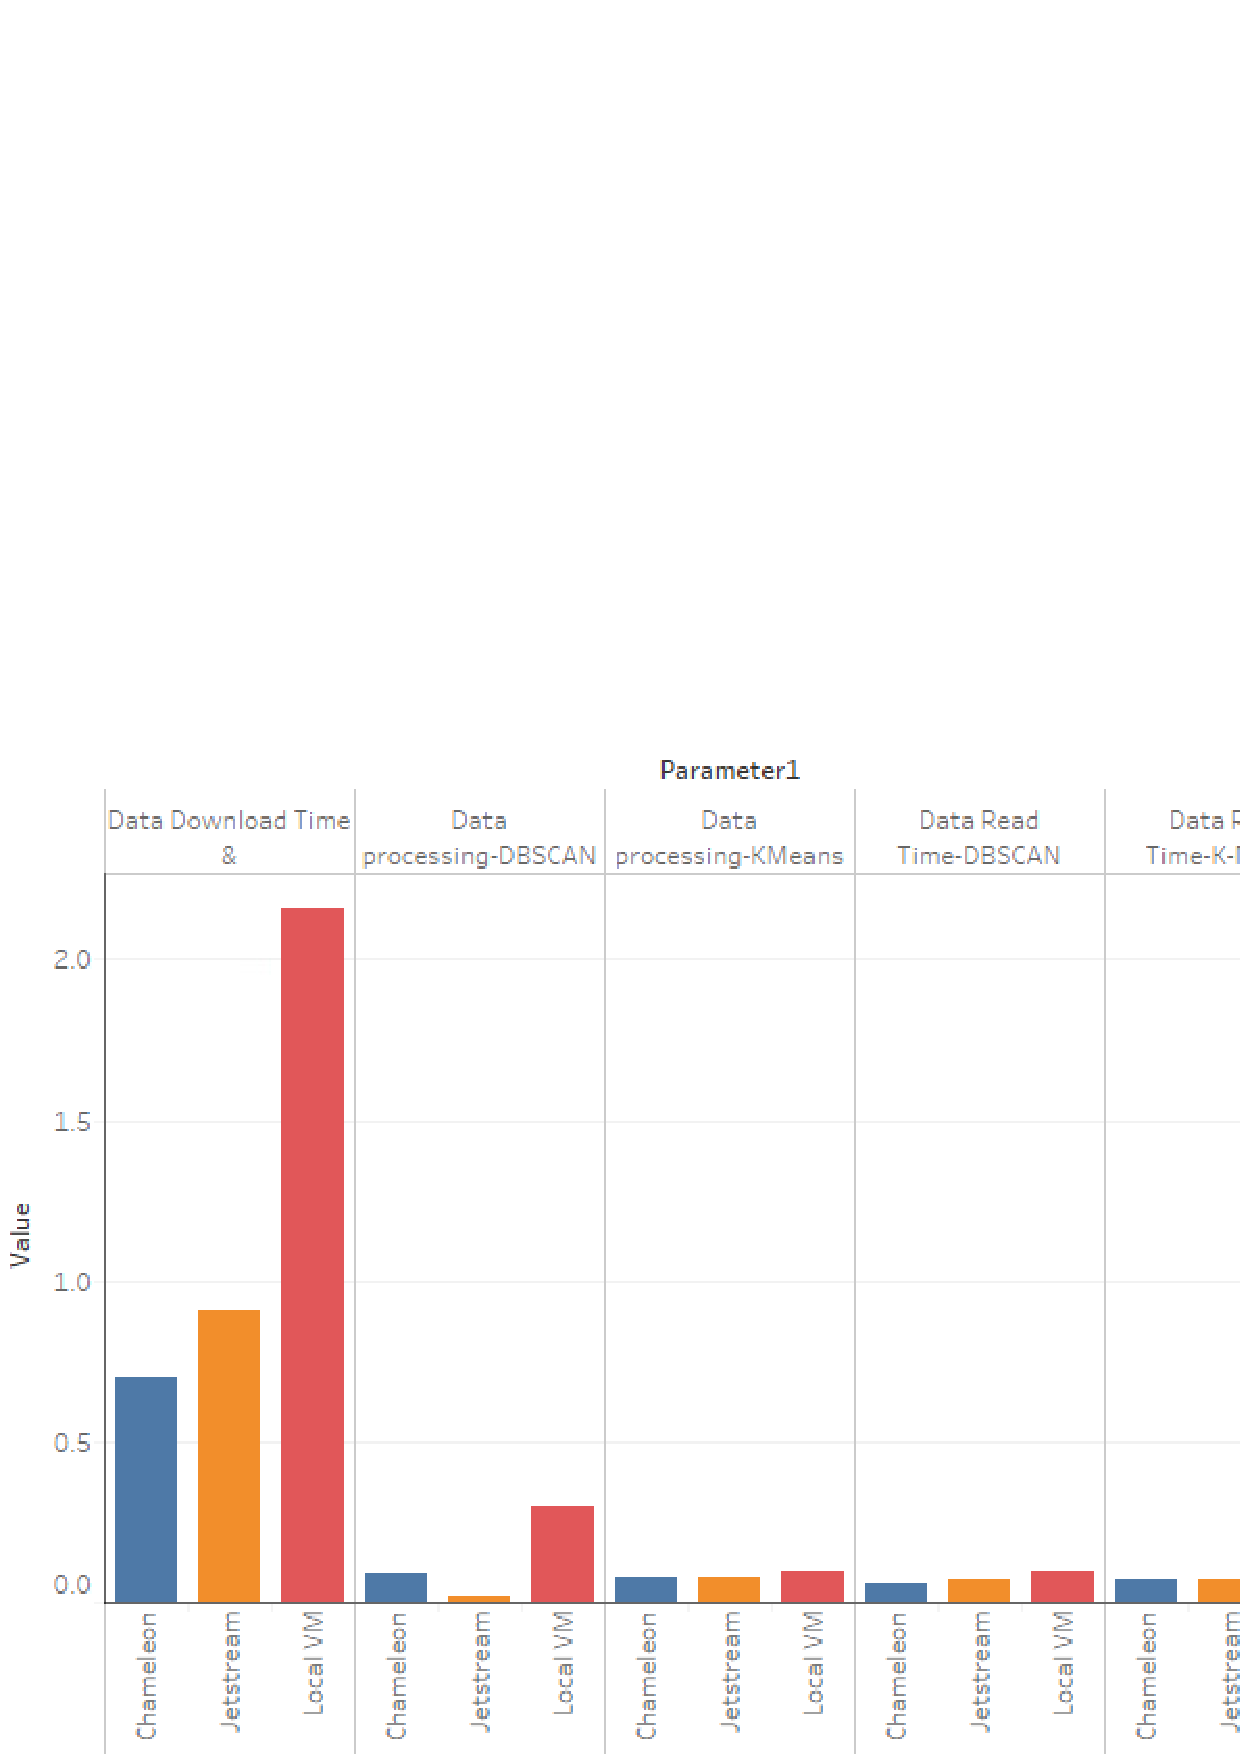
\includegraphics[width=\linewidth]{images/figure2}}
\caption{Time taken for small dataset} 
\label{fig:figure2}
\end{figure}


\begin{figure}[htbp]
\centering
\fbox{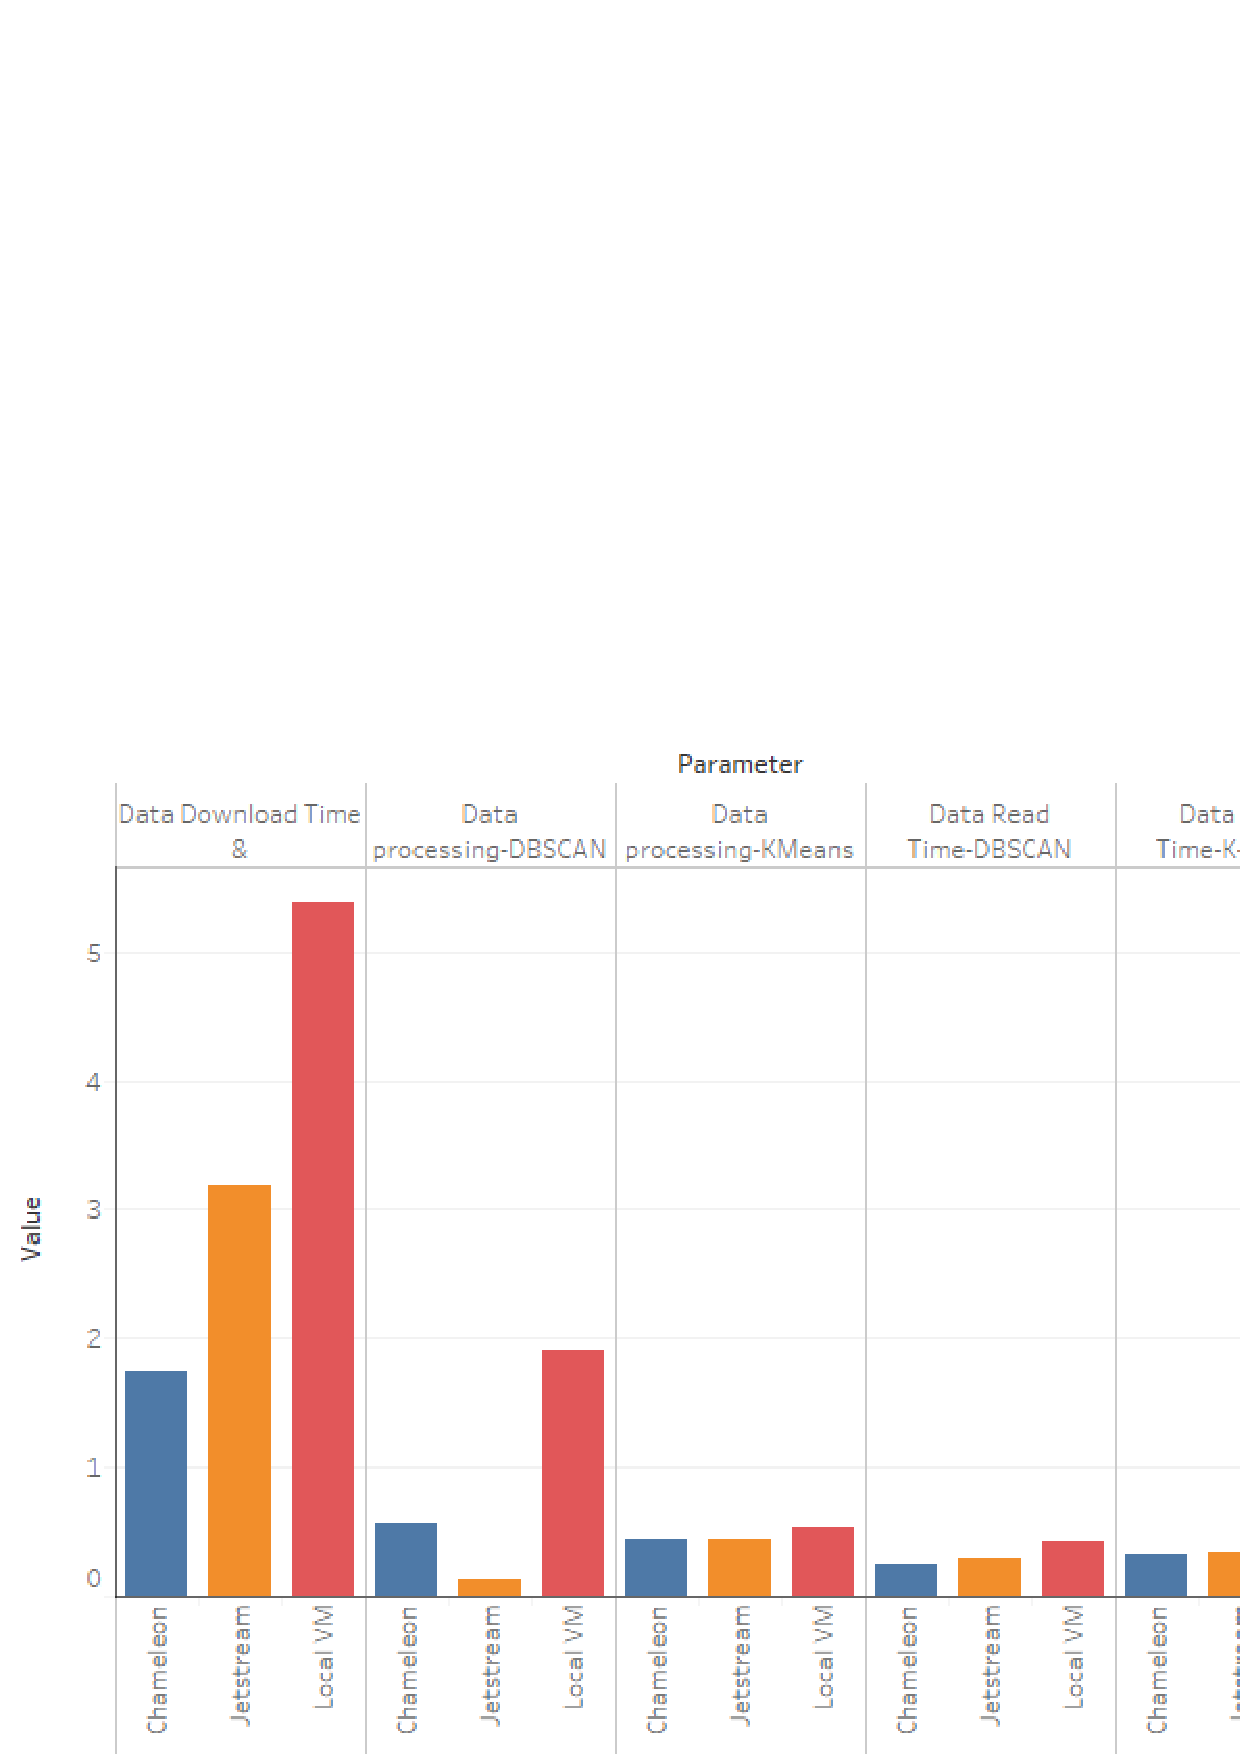
\includegraphics[width=\linewidth]{images/figure3}}
\caption{Time taken for large dataset} 
\label{fig:figure3}
\end{figure}

\section {Result And Analysis}

Figure \ref{fig:figure1} shows default page showing application usage. Output of K-Means clustering of magnitude and depth data is given in Figure 5. Figure 6 shows a closer look at scatter plot. Figure 7 is the output of DBSCAN clustering of earthquake locations. Both the graphs are interactive. On the 'Magnitude and Depth' graph one can choose one or more clusters. Mouse hover shows magnitude  and its corresponding depth. The 'Earthquake locations' globe shows lat-long information on mouse hover. The user can rotate the globe with mouse key press.


\begin{figure}[htbp]
\centering
\fbox{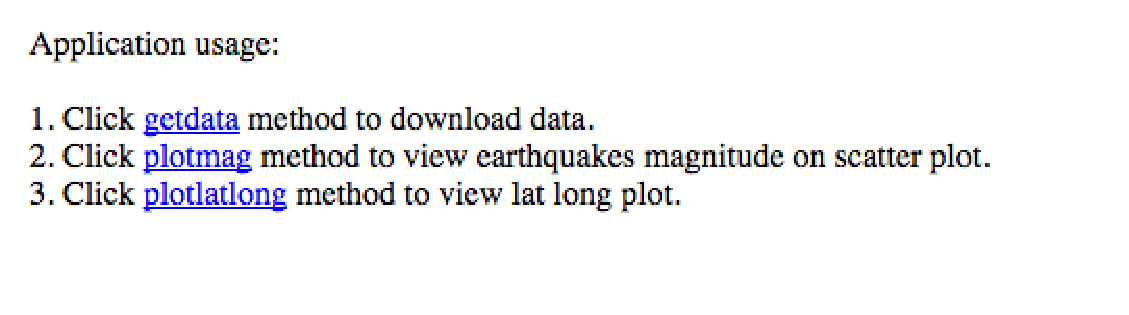
\includegraphics[width=\linewidth]{images/figure1}}
\caption{Application usage} 
\label{fig:figure1}
\end{figure}

\begin{figure}[htbp]
\centering
\fbox{\includegraphics[width=\linewidth]{images/figure5}}
\caption{Magnitude and Depth(Kms)} 
\label{fig:figure5}
\end{figure}


\begin{figure}[htbp]
\centering
\fbox{\includegraphics[width=\linewidth]{images/figure6}}
\caption{Close look at the cluster} 
\label{fig:figure6}
\end{figure}


\begin{figure}[htbp]
\centering
\fbox{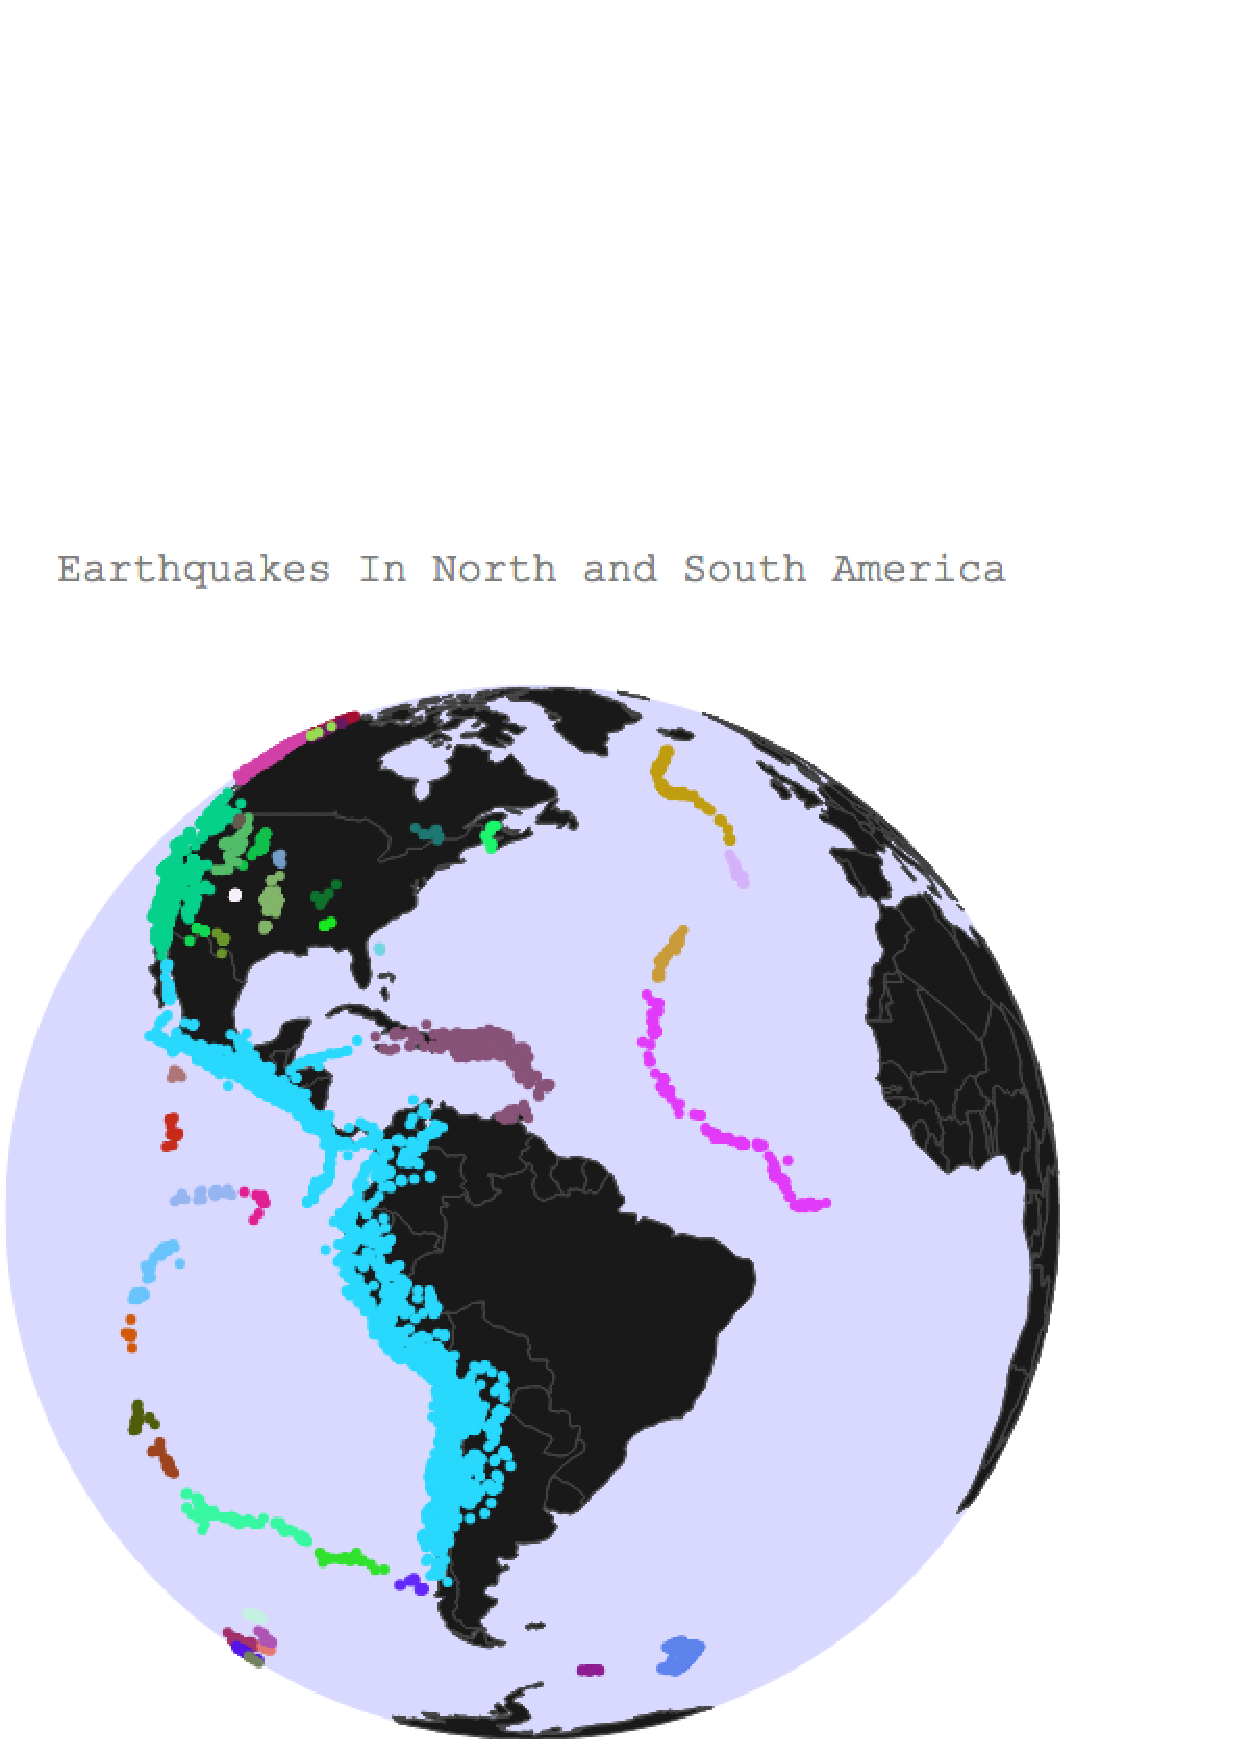
\includegraphics[width=\linewidth]{images/figure7}}
\caption{Earthquake locations on globe} 
\label{fig:figure7}
\end{figure}

The focus of an earthquake is the actual point underground where rocks break. From the results it is clear that there were fewer earthquakes having the focus deep, greater than 300kms. Earthquakes having shallow focus (less than 70kms) are comparatively lesser than the ones having intermediate focus (70kms to 300km). Thus, maximum earthquakes occurred between 70kms to 300kms deep underground.

Analysis of earthquake locations shows that maximum earthquakes have happened in the Pacific coastal area of North and south America. We can confirm this result with USGS facts, which states "The majority of the earthquakes and volcanic eruptions occur along plate boundaries such as the boundary between the Pacific Plate and the North American plate. One of the most active plate boundaries where earthquakes and eruptions are frequent, for example, is around the massive Pacific Plate commonly referred to as the Pacific Ring of Fire \cite{www-usgs4}."

There is a subtle difference in output of K-Means and DBSCAN algorithms. K-Means worked with lesser number of clusters (3), while DBSCAN created greater number of clusters, more than 50 in this case. K-Means produced output linearly, cluster1 to cluster3. DBSCAN produced non-linear output. A cluster in Pacific ocean is Cluster28, whereas, the cluster adjacent to it is Cluster39.  


\section {Conclusion}
This project was an opportunity to use Big Data open source software and projects. 
We can conclude that Ansible is a powerful tool for one click deployment and continuous integration. Cloudmesh client is a convenient tool to work with multiple cloud environments at the same time. Plotly is a powerful library that allows creating interactive visualization. 

While researching for the algorithms we came to know that DBSCAN is better choice for classification if one doesn't want to specify number of clusters beforehand.

Analysis of earthquakes data showed interesting facts. In 2 years span from year 2015 till 2017 there were around 15,000 earthquakes of magnitude more than 3, and approx 7,100 earthquakes of magnitude more than 4.

\section {Acknowledgements}

This project is undertaken as part of the I524: Big Data and Open Source Software Projects course at Indiana University. The author would like to thank Prof. Gregor von Laszewski and his associates from the School of Informatics and Computing for providing all the technical support and assistance.

\section {Licensing}

Project uses Apache license ver 2.0.


% Bibliography

\bibliography{references}
 
\newpage

\section{Appendices}

Appendix A: The work on this project was distributed as follows between the
authors:

\begin{description}

\item[Nandita Sathe.] She completed all the work related to development of this application including research, testing and writing the project report. 

\end{description}

\end{document}
